% Options for packages loaded elsewhere
\PassOptionsToPackage{unicode}{hyperref}
\PassOptionsToPackage{hyphens}{url}
%
\documentclass[
]{book}
\usepackage{lmodern}
\usepackage{amsmath}
\usepackage{ifxetex,ifluatex}
\ifnum 0\ifxetex 1\fi\ifluatex 1\fi=0 % if pdftex
  \usepackage[T1]{fontenc}
  \usepackage[utf8]{inputenc}
  \usepackage{textcomp} % provide euro and other symbols
  \usepackage{amssymb}
\else % if luatex or xetex
  \usepackage{unicode-math}
  \defaultfontfeatures{Scale=MatchLowercase}
  \defaultfontfeatures[\rmfamily]{Ligatures=TeX,Scale=1}
\fi
% Use upquote if available, for straight quotes in verbatim environments
\IfFileExists{upquote.sty}{\usepackage{upquote}}{}
\IfFileExists{microtype.sty}{% use microtype if available
  \usepackage[]{microtype}
  \UseMicrotypeSet[protrusion]{basicmath} % disable protrusion for tt fonts
}{}
\makeatletter
\@ifundefined{KOMAClassName}{% if non-KOMA class
  \IfFileExists{parskip.sty}{%
    \usepackage{parskip}
  }{% else
    \setlength{\parindent}{0pt}
    \setlength{\parskip}{6pt plus 2pt minus 1pt}}
}{% if KOMA class
  \KOMAoptions{parskip=half}}
\makeatother
\usepackage{xcolor}
\IfFileExists{xurl.sty}{\usepackage{xurl}}{} % add URL line breaks if available
\IfFileExists{bookmark.sty}{\usepackage{bookmark}}{\usepackage{hyperref}}
\hypersetup{
  pdftitle={ Democratizando a Bioinformática },
  pdfauthor={Kelly Hidalgo, Tiago Palladino, Victor Borin, Carla Paixão, Valéria Maia Merzel},
  hidelinks,
  pdfcreator={LaTeX via pandoc}}
\urlstyle{same} % disable monospaced font for URLs
\usepackage{longtable,booktabs}
\usepackage{calc} % for calculating minipage widths
% Correct order of tables after \paragraph or \subparagraph
\usepackage{etoolbox}
\makeatletter
\patchcmd\longtable{\par}{\if@noskipsec\mbox{}\fi\par}{}{}
\makeatother
% Allow footnotes in longtable head/foot
\IfFileExists{footnotehyper.sty}{\usepackage{footnotehyper}}{\usepackage{footnote}}
\makesavenoteenv{longtable}
\usepackage{graphicx}
\makeatletter
\def\maxwidth{\ifdim\Gin@nat@width>\linewidth\linewidth\else\Gin@nat@width\fi}
\def\maxheight{\ifdim\Gin@nat@height>\textheight\textheight\else\Gin@nat@height\fi}
\makeatother
% Scale images if necessary, so that they will not overflow the page
% margins by default, and it is still possible to overwrite the defaults
% using explicit options in \includegraphics[width, height, ...]{}
\setkeys{Gin}{width=\maxwidth,height=\maxheight,keepaspectratio}
% Set default figure placement to htbp
\makeatletter
\def\fps@figure{htbp}
\makeatother
\setlength{\emergencystretch}{3em} % prevent overfull lines
\providecommand{\tightlist}{%
  \setlength{\itemsep}{0pt}\setlength{\parskip}{0pt}}
\setcounter{secnumdepth}{5}
\usepackage{booktabs}
\ifluatex
  \usepackage{selnolig}  % disable illegal ligatures
\fi
\usepackage[]{natbib}
\bibliographystyle{apalike}

\title{ Democratizando a Bioinformática}
\author{Kelly Hidalgo, Tiago Palladino, Victor Borin, Carla Paixão, Valéria Maia Merzel}
\date{2021-03-23}

\begin{document}
\maketitle

{
\setcounter{tocdepth}{1}
\tableofcontents
}
\hypertarget{prefacio}{%
\chapter*{Prefacio}\label{prefacio}}
\addcontentsline{toc}{chapter}{Prefacio}

\begin{center}\rule{0.5\linewidth}{0.5pt}\end{center}

\begin{center}
\includegraphics[width=1.2\linewidth,height=1.2\textheight]{imgs/1} \end{center}

Esta é um guia *simples\textbf{ e }didático** para se inciar no mundo da bioinformática para processamento e análises de sequenciamento em grande escala. No primeiro volume serão abordadas as análises de sequênciamento do amplicon do gene 16S rRNA pela plataforma \emph{Illumina}.

\hypertarget{por-que-lerusar-este-livro}{%
\section*{Por que ler/usar este livro?}\label{por-que-lerusar-este-livro}}
\addcontentsline{toc}{section}{Por que ler/usar este livro?}

Este livro foi pensando para ajudar pessoas que tem pouca ou nenhuma experiência com bioinformática e no seus trabalhos ou projetos precisam analisar dados de microbiomas obtidos a partir de sequenciamento em larga escala, especialmente na plataforma Illumina. É um guia teórico/prático para processar este tipo de dados com total independência.

Foi criado a partir da experiencia dos autores, quem também tiveram que enfrentar dificuldades para iniciar com este tipo de análises e pensando em isto desenvolveram o presente guía para ajudar a novos iniciantes.

\hypertarget{estrutura-do-livro}{%
\section*{Estrutura do livro}\label{estrutura-do-livro}}
\addcontentsline{toc}{section}{Estrutura do livro}

O primeiro volume, está dividido em três grandes partes. A primeira tem uma introdução ao mundo das linguagens de programação, onde serão introduzidos os comandos mais básicos para se desenvolver na linha de comando. A segunda parte contempla o processamento de dados de sequenciamento do amplicon 16S rRNA, desde a obtenção dos dados, passando pelo controle de qualidade, a eliminação de quimeras, clusterização em ASV (\emph{Amplicon sequence variant}) e anotação taxonômica, usando três ferramentas diferentes (\emph{Qiime2}, \emph{DADA2}, \emph{Galaxy}) . Por último, são abordadas as análises para geração de gráficos e estatísticas utilizando principalmente a linguagem \textbf{R}, no entanto também são aprensentadas outras alternativas.

\hypertarget{informauxe7uxe3o-sobre-software-e-convenuxe7uxf5es}{%
\section*{Informação sobre software e convenções}\label{informauxe7uxe3o-sobre-software-e-convenuxe7uxf5es}}
\addcontentsline{toc}{section}{Informação sobre software e convenções}

O conteúdo de este livro será principalmente para usuários de Linux/MacOs. Para os usuários de Windows, se recomenda, instalar um programa ou aplicativo para aceder a um servidor com Linux (p.e. \emph{MobaXterm}, \emph{Putty}, \emph{Secure Shell App de Google Chrome Apps}) ou instalar uma maquina virtual com Linux (recomendada \textbf{Ubuntu}). No entanto é sempre recomendável revisar a configuração do computador a ser usado e conferir que cumpre com os requisitos mínimos de cada software.

Os \emph{pipelines} de este livro usam diversos software, que irão se apresentando na medida que sejam necessários. A maioria das ferramentas baseadas em código (\emph{code based}), serão instaladas usando \href{https://anaconda.org/bioconda}{Bioconda`s package} de \href{https://anaconda.org/}{Anaconda}.

O software \textbf{R} será bastante usado durante várias etapas do processamento e análises de dados. Se recomenda a instalação \emph{R version 4.0.4} e o IDLE \emph{RStudio} a versão mais recente. (\textbf{Nota:} A instalação destes software será abordada em seções mais para frente).

\hypertarget{convenuxe7uxf5es}{%
\subsubsection*{Convenções}\label{convenuxe7uxf5es}}
\addcontentsline{toc}{subsubsection}{Convenções}

\begin{center}\rule{0.5\linewidth}{0.5pt}\end{center}

Não será adicionados \textbf{prompts} (i.e.~\texttt{\textgreater{}} e \texttt{+}) aos códigos em este livro. Os comentários dentro dos códigos serão sinalizados com \texttt{\#\#}. Os nomes de ferramentas, softwares e pacotes serão escritos em negrita (p.e. \textbf{Qiime2}), e código na linha serão formatados em fonte typewriter (p.e. \texttt{qiime2\ -h}).

Em construção\ldots{}

\hypertarget{agradecimentos}{%
\section*{Agradecimentos}\label{agradecimentos}}
\addcontentsline{toc}{section}{Agradecimentos}

Em construção\ldots{}

\hypertarget{acerca-dos-autores}{%
\chapter*{Acerca dos autores}\label{acerca-dos-autores}}
\addcontentsline{toc}{chapter}{Acerca dos autores}

\begin{center}\rule{0.5\linewidth}{0.5pt}\end{center}

\hypertarget{msc.-kelly-hidalgo}{%
\paragraph*{MsC. Kelly Hidalgo}\label{msc.-kelly-hidalgo}}
\addcontentsline{toc}{paragraph}{MsC. Kelly Hidalgo}

\begin{center}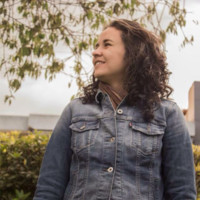
\includegraphics[width=0.4\linewidth,height=0.4\textheight]{imgs/KellyHidalgo} \end{center}

Kelly atualmente é doutoranda do programa de Genética e Biologia Molecular da Universidade Estadual de Campinas. Desenvolve seu projeto de doutorado no \emph{Centro Plurisdisciplinar de Pesquisa Químicas, Biológicas e Agricolas} (CPQBA - UNICAMP), na divisão de Recursos Microbianos no \textbf{Grupo de Ecologia Microbiana e Multi-ômicas} dirigido pela Doutora Valéria Maia Merzel.
Kelly pesquisa principalmente sobre ambientes contaminados com petróleo ou derivados, abordagens de biorremediação, impacto da contaminação com microrganismos na industria petrolifera, usando multi-ômicas para melhor compreensão dos procesos microbiológicos que acontecem em estes ambientes.

\href{https://orcid.org/0000-0003-4607-3750}{
\includegraphics{imgs/orcid.png}} \href{https://github.com/khidalgo85}{
\includegraphics{imgs/github.png}}

  \bibliography{book.bib,packages.bib}

\end{document}
